\newpage
\section{Modelowanie obiektów 3D}
\subsection{Bazowa aplikacja}
Aplikacja bazowa, po zainicjowaniu niezbędnych elementów biblioteki \textit{GLUT}, oddaje sterowanie do utworzonej klasy \lstinline{ViewEngine}. Przechowuje one referencje na klasy, będące niezależnymi widokami. Widoki te posiadają zdefiniowane własne funkcje odpowiedzialne za renderowanie, obsługę zdarzeń, animację oraz obsługę zdarzeń związanych z~cyklem życia widoku. Poprzez zmianę wartości wskaźnika na aktualny widok w klasie \lstinline{ViewEngine}, funkcje przekazane do biblioteki \textit{GLUT} zastępowane są funkcjami właściwego widoku. Każdy widok musi implementować interfejs \lstinline{iView} zdefiniowany następująco:

\begin{lstlisting}[language=C++, caption=Interfejs IView.]
class IView
{
public:
    virtual std::string getName() = 0;
    virtual void init() = 0;
    virtual void onEnter() = 0;
    virtual void render() = 0;
    virtual void idle() = 0;
    virtual void timer() = 0;
    virtual void onKey(unsigned char key, int x, int y) = 0;
    virtual void onLeave() = 0;

    virtual ~IView(){};
};
\end{lstlisting}
Widoku identyfikowane są za pomocą nazw zwracanych przez funkcję \lstinline{getName()}.
Dzięki zaimplementowaniu wzorca Singleton w klasie \lstinline{ViewEngine} możliwe jest przełączanie widoku w dowolnym miejscu wywołania metody w programie.
\begin{lstlisting}[language=C++, caption=Tworzeznie instancji widoków i~ustawianie obecnego. Funkcja \lstinline{g} zwraca instancję klasy.]
ViewEngine::g().add(new TeapotView());
ViewEngine::g().add(/*inne widoki*/);
ViewEngine::g().setCurrent("complexEgg");
\end{lstlisting}
\subsection{Model i~generowanie punktów}
\subsubsection{Generowanie punktów}
W ćwiczeniu wygenerowane zostały punkty modelu jajka. Uzyskane zostały poprzez obrócenie odpowiednio dobranej krzywej Beziera. Punkty opisują wzory w dziedzinie parametrycznej kwadratu jednostkowego:
\begin{align*}
    x(u,v)&=(-90u^5+225u^4-270u^3+180u^2-45u)cos(\pi v)\\
    y(u,v)&=160u^4-320u^3+160u^2\\
    z(u,v)&=(-90u^5+225u^4-270u^3+180u^2-45u)sin(\pi v)
\end{align*}
Generowanie punktów dla wartości parametrów funkcji z~przedziału $<0;1>$ zakłada wygenerowanie nakładających się punktów. Dlatego w programie pominięto ostatnie iteracje pętli.
\subsubsection{Model}
Każdy model zdefiniowany jest za pomocą klasy, która przyjmuje parametry określające jego wygląd i~zachowania. W przypadku klasy \lstinline{Egg} jest to ilość iteracji pętli generowania punktów, co przekłada się na poziom wygładzenia modelu. Klasa modelu odpowiedzialna jest również za jego rysowanie w różnych wariantach.

Dla czytelności kodu stworzona została klasa \lstinline{Point}, która przechowuje współrzędne punktu, jego kolor, oraz odpowiedzialna jest rysowanie samego siebie.

\begin{lstlisting}[language=C++, caption=Nagłówek klasy Point.]
class Point
{
public:
    Point(float x, float y, float z, GLubyte r, GLubyte g, GLubyte b)
        : color({r, g, b}), x(x), y(y), z(z){};
    ~Point();
    void callGlVertex3f();
    void callGlColor3f();
    void drawWithColor();
    struct Color
    {
        GLubyte r = 255;
        GLubyte g = 255;
        GLubyte b = 255;
    };
    float x = 0;
    float y = 0;
    float z~= 0;
    Color color;
};
\end{lstlisting}
Właściwa generacja punktów odbywa się w konstruktorze klasy \lstinline{Egg}.
\begin{lstlisting}[language=C++, caption=Nagłówek klasy modelu Egg.]
class Egg
{
public:
    Egg(int n = 32);
    ~Egg();
    std::vector<std::vector<Point>> getPoints();
    void renderPoints();
    void renderMesh();
    void renderTriangles();
    void renderComplex();
private:
    int n;
    std::vector<std::vector<Point>> points;
    float calcX(float u, float v);
    float calcY(float u, float v);
    float calcZ(float u, float v);
};
\end{lstlisting}
\newpage
\subsection{Rysowanie modelu za pomocą punktów, siatki i~jako bryły}

W utworzonej aplikacji rysowanie odbywa się w metodzie \lstinline{IView::render()} modelu. Znajduje się tam również opisana niżej procedura transformacji i~animacji modelu.
\subsubsection{Rysowanie punktów}
Rysowanie punktów obywa się z~wykorzystanie prymitywu \lstinline{GL_POINTS} biblioteki \textit{OpenGL}. Wszystkie punkty podawane są do funkcji w dowolnej kolejności.

\begin{lstlisting}[label={lst:anim}, language=C++, caption=Rysowanie jajka z~punktów. Widok \lstinline{DottEggView}]
void DotEggView::render()
{
    glLoadIdentity();
    glRotated(eggRotation, 1, 1, 1);
    glTranslated(0, -5., 0);
    glPointSize(10.);
    egg.renderPoints();
}
\end{lstlisting}
\begin{lstlisting}[language=C++, caption=Rysowanie jajka z~punktów. Model \lstinline{Egg}]
void Egg::renderPoints()
{
    glBegin(GL_POINTS);
    for (auto &&row : points)
    {
        for (auto &&point : row)
        {
            point.drawWithColor();
        }
    }
    glEnd();
}
\end{lstlisting}
\newpage
\subsection{Rysowanie siatki i~bryły}
Rysowanie siatki i~bryły odbywa się analogicznie do rysowania punktów. Jedyną różnicą jest użyty prymityw, oraz kolejność umieszczania punktów, która różni się w zależności od prymitywu. Dla siatki użyty został prymityw \lstinline{GL_LINES}. Bryła została narysowana na dwa sposoby używając prymitywów \lstinline{GL_TRIANGLES} i~\lstinline{GL_TRIANGLE_STRIP}, co po narysowaniu daje taki sam efekt.

\begin{figure}[H]
    \
    \begin{minipage}[t]{.45\linewidth}
        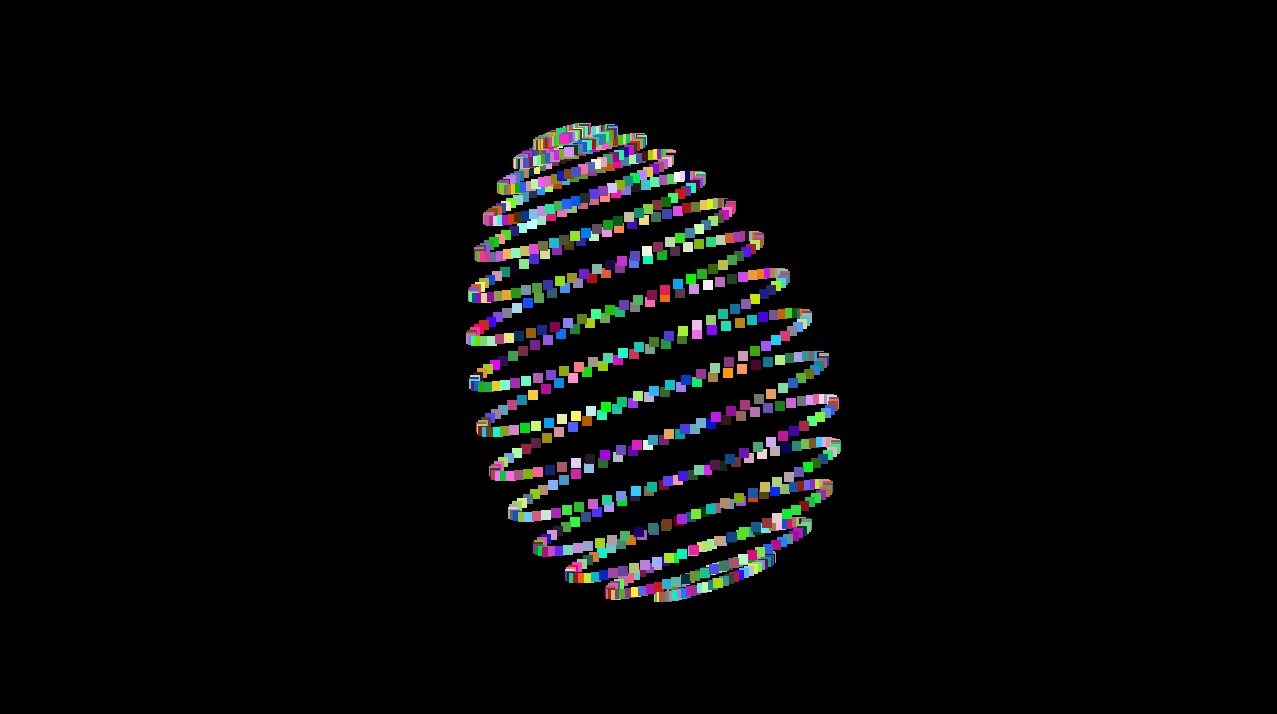
\includegraphics[width=\linewidth, trim={8cm 0 8cm 0},clip]{img/egg_1.png}
        \caption{Model jajka zbudowany z~punktów.}
    \end{minipage}
    \hspace{.05\linewidth}
    \begin{minipage}[t]{0.45\linewidth}
        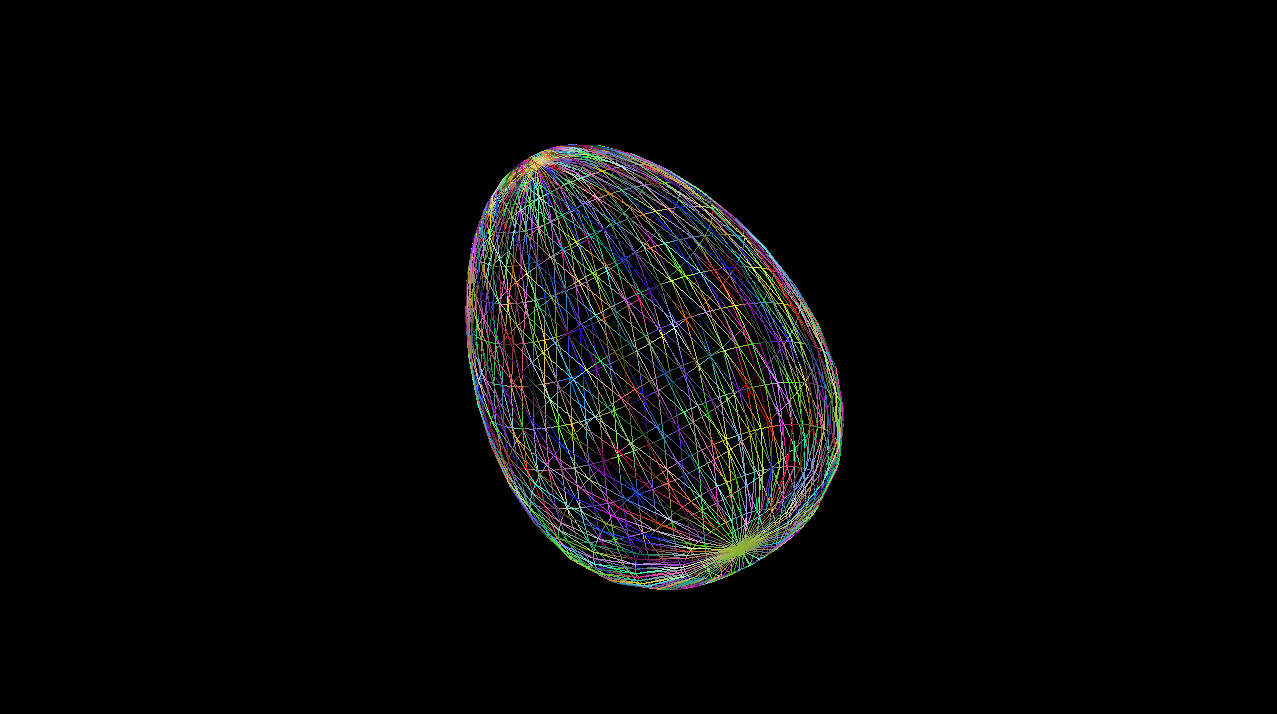
\includegraphics[width=\linewidth, trim={8cm 0 8cm 0},clip]{egg_2}
        \caption{Model jajka zbudowany z~siatki.}
    \end{minipage}
\end{figure}
\begin{figure}[h]
    \centering
    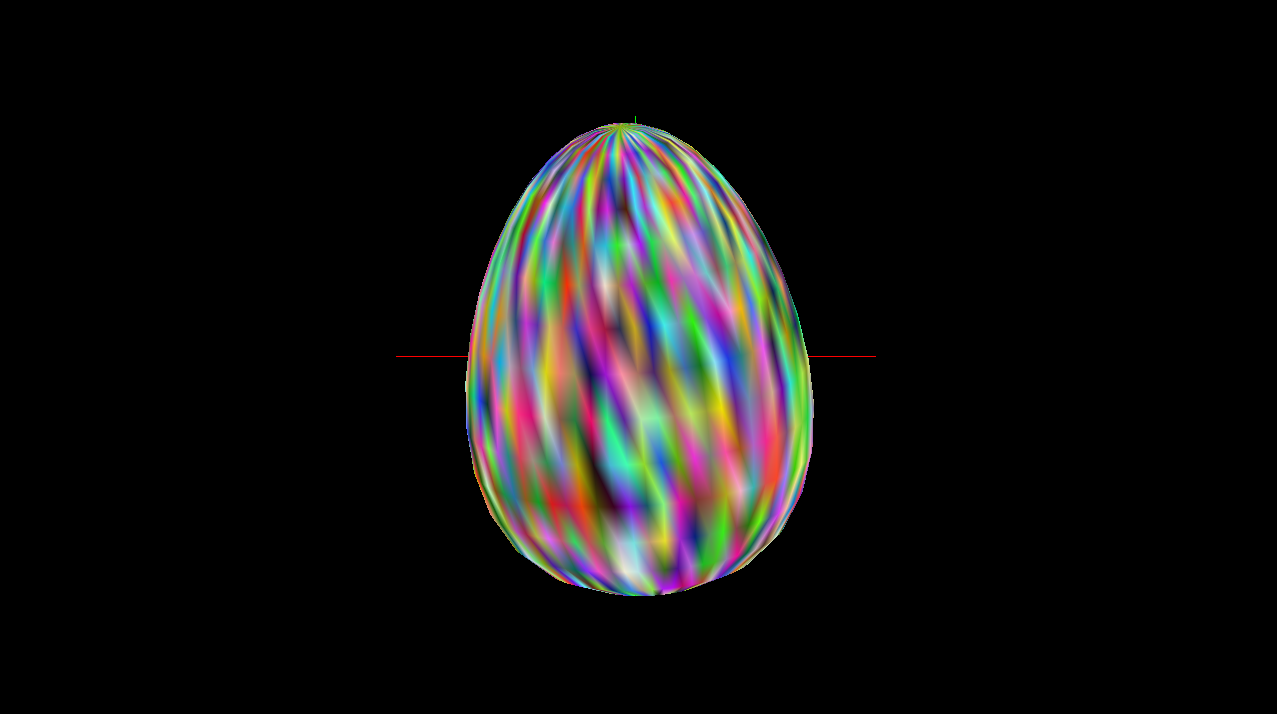
\includegraphics[width=0.45\linewidth, trim={8cm 0 8cm 0},clip]{img/egg_3.png}
    \caption{Model jajka zbudowany z~trójkątów.}
\end{figure}
\newpage
W przypadku rysowania za pomocą siatki wymagane było ujednolicenie losowo generowanych kolorów dla punktów, które w procesie ich generowania się na siebie nakładają. Ma to miejsce na czubkach oraz, w przypadku generowania dla całego zakresu $<0;1>$, dla jednego z \textit{południków} jajka.

\subsection{Animacja obrotu}
Zmiana kąta obrotu modelu odbywa się w metodzie \lstinline{IView::timer()} widoku, która wywoływana jest 60 razy na sekundę korzystając z funkcji \lstinline{void glutTimerFunc(unsigned int time, void (*callback)(int), int value)}. Zapewnia to większą kontrolę nad animacją i jej prędkością niż podanie wskaźnika do funkcji \lstinline{void glutIdleFunc(void (*callback)())}.
Metoda widoku inkrementuje zmienną definiującą kąt obrotu modelu dla rysowanej klatki. W listingu \ref{lst:anim}, podczas rysowania, przeprowadzony jest proces transformacji modelu. Najpierw resetowana jest macierz transformacji, potem dokonywany jest obrót o wartość ze zmiennej widoku wokół wszystkich osi. Translacja w osi $Y$ ustawia model \textit{mniej więcej} po środku ekranu.
\begin{lstlisting}[language=C++, caption=Ustawianie zmiennej kątu obrotu i przerysowanie klatki.]
void DotEggView::timer()
{
    eggRotation += 1;
    if (eggRotation >= 360)
        eggRotation = 0;
    glutPostRedisplay();
}
\end{lstlisting}
